%-------------------------------------------------------------------
% bachelor thesis
% create by: Mario Preishuber
% create date: 2014, Jan 01.
%-------------------------------------------------------------------

\section{System vs. Mutator} \label{sec:analysis_sys_vs_mut}

In the previous sections we described our analysis results separated in system heap and mutator heap. We presented the differences and similarities distinguished by the type of the objects. In this section we compare system and mutator objects and do not care about the type of the objects. As explained in Section \ref{sec:analysis_mutator} are objects of type array, string, user-defined object, code, closure, regular expression (regexp), or number are mutator objects. Objects of type hidden, native, or synthetic are system objects as described in Section \ref{sec:analysis_system}. The comparison of system an mutator illustrates the overhead produced by Google's V8. 

Figure \ref{fig:obj_sysmut_alloc_dist} shows a histogram of the object distribution for all workloads. On the x-axis the workloads are listed and on the y-axis the relative amount of objects is displayed. The histogram shows that about 25\% of the allocated objects are system objects. As explained in Section \ref{sec:analysis_system} most of these objects are of type hidden. We conclude that nearly 25\% of all allocated objects are used for the internal representation of objects.
\begin{figure}
	\centering
	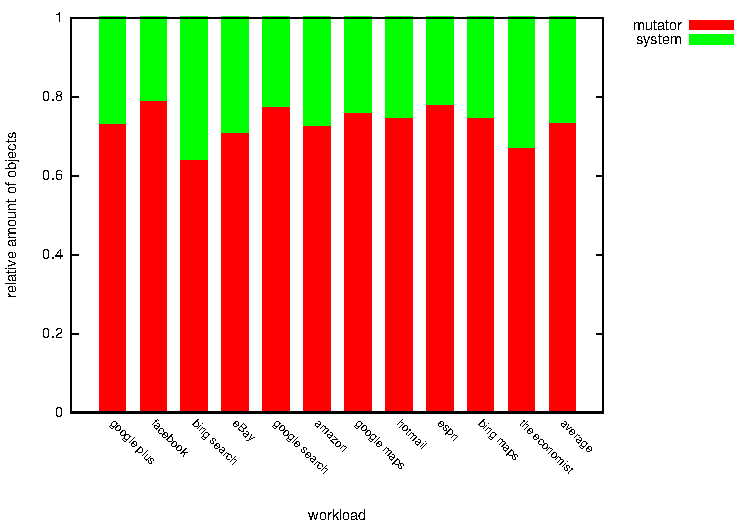
\includegraphics[width=0.5\textwidth]{obj_sysmut_alloc_dist}
	\caption{Histogram of the object distribution for all workloads.}
	\label{fig:obj_sysmut_alloc_dist}
\end{figure}

The distribution of the out-degree is presented by Figure \ref{fig:obj_sysmut_outdeg_dist}. On the x-axis is the out-degree shown and on the y-axis the relative amount of objects with an out-degree smaller than x is presented. Figure \ref{fig:obj_sysmut_outdeg_dist} shows a quite different behavior of system and mutator objects. The only similarity is that there are few objects with an out-degree higher than six. More detailed, there are less than 1\% of system and less than 10\% of mutator objects with a higher out-degree than six. It is also interesting that the out-degree of mutator objects is significantly smaller as the out-degree of system objects.
\begin{figure}
	\centering
	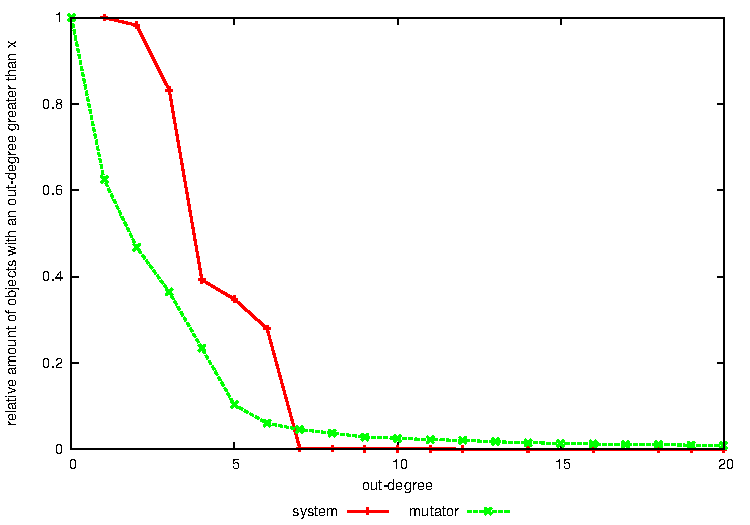
\includegraphics[width=0.5\textwidth]{obj_sysmut_outdeg_dist}
	\caption{Out-degree distribution of real web applications.}
	\label{fig:obj_sysmut_outdeg_dist}
\end{figure}

The lifetime distribution, illustrated by Figure \ref{fig:obj_sysmut_lieftiem_dist}, presents a similar behavior of system and mutator objects. A reason for this is the dependency of hidden classes and user-define objects and again the fact that most of the system objects are of the type hidden. On the x-axis of the figure the object lifetime in allocated KB is shown and on the y-axis the relative amount of objects living shorter than x is displayed. 
\begin{figure}
	\centering
	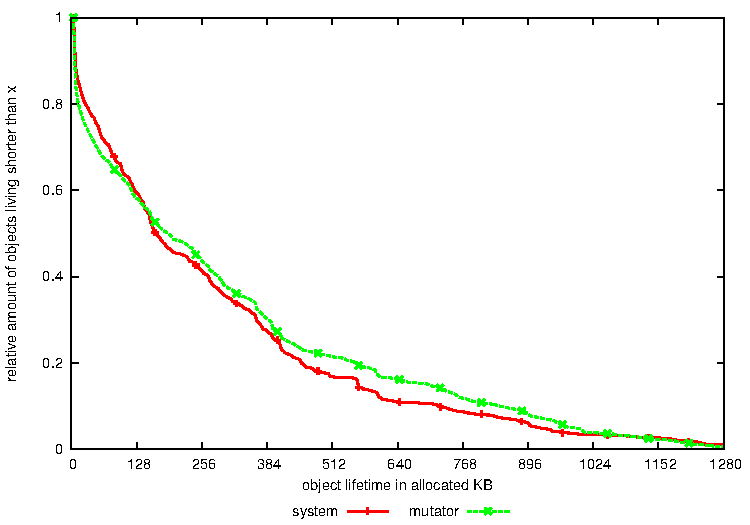
\includegraphics[width=0.5\textwidth]{obj_sysmut_lifetime_dist}
	\caption{Lifetime distribution of real web applications.}
	\label{fig:obj_sysmut_lieftiem_dist}
\end{figure}

Figure \ref{fig:obj_sysmut_rootdist_dist} presents the distribution of the root distance of all snapshots of all workloads separated in system and mutator objects. On the x-axis the minimum root distance is shown and on the y-axis the relative amount of objects with a root distance smaller than x is shown. The behavior of the system and mutator objects is extremely similar. We conclude that there might be a dependency of the position of system objects and the position of mutator objects in a heap graph. A reason could be that a user-defined objects has a reference the hidden class which represents the properties of a object.  
\begin{figure}
	\centering
	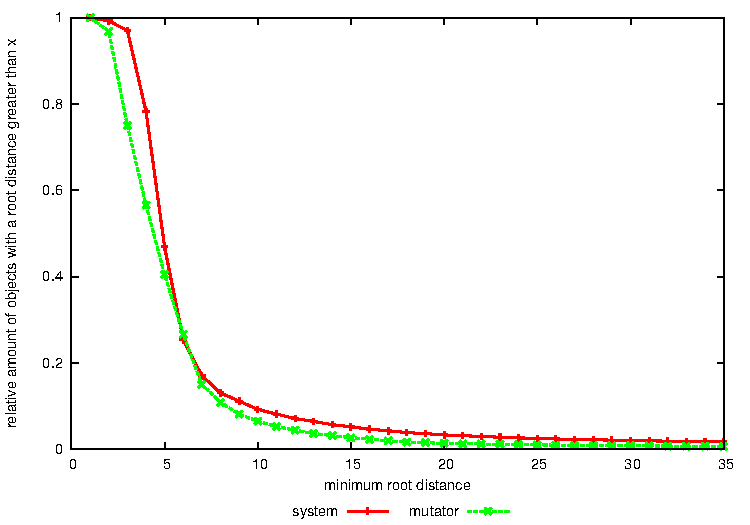
\includegraphics[width=0.5\textwidth]{obj_sysmut_rootdist_dist}
	\caption{Root distance distribution of real web applications.}
	\label{fig:obj_sysmut_rootdist_dist}
\end{figure}

If we compare the size distribution of system and mutator objects we recognize that system objects are significantly bigger. This behavior is illustrated by Figure \ref{fig:obj_sysmut_selfsize_dist}, which shows on the x-axis the size in byte and on the y-axis relative amount of objects smaller than size x.
\begin{figure}
	\centering
	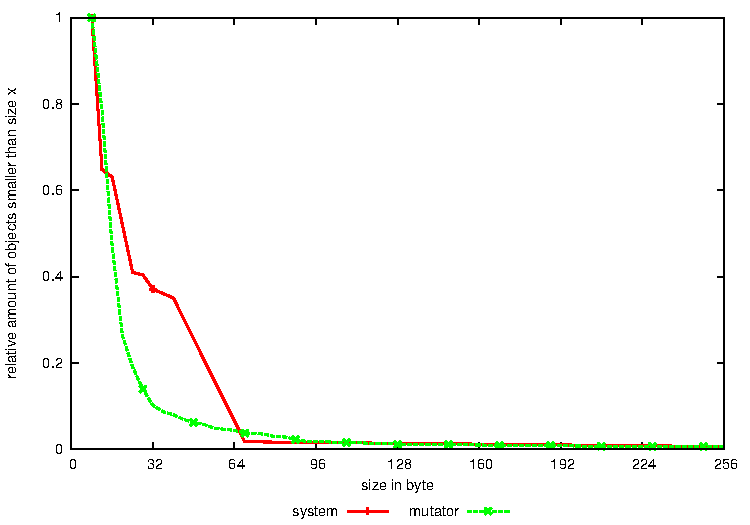
\includegraphics[width=0.5\textwidth]{obj_sysmut_selfsize_dist}
	\caption{Size distribution of real web applications.}
	\label{fig:obj_sysmut_selfsize_dist}
\end{figure}